\documentclass[a4paper,10pt]{article}
\usepackage[spanish]{babel} % Traduce cosas como "February" o "References" por "Febrero" / "Referencias"
\usepackage[utf8]{inputenc}

\usepackage{fancyvrb}
\usepackage{graphicx}
\graphicspath{ {graficos/} }

\usepackage{float}
\usepackage[colorlinks=true,linkcolor=black,urlcolor=blue,bookmarksopen=true]{hyperref}
\usepackage{bookmark}
\usepackage{fancyhdr}
\usepackage{bbm}
\usepackage{amssymb}
\usepackage{amsmath}
\usepackage{subcaption}
\usepackage{graphicx}
\usepackage{lipsum}
\usepackage{wrapfig}
\usepackage{csquotes}
\usepackage{xcolor}
\usepackage[legalpaper, portrait, margin=1.5in]{geometry}

\newcommand{\argmin}{\operatornamewithlimits{argmin}}


\pagestyle{fancy} % Encabezado y pie de página
\fancyhf{}
\fancyhead[L]{}
\fancyhead[R]{86.36 / 66.69 Criptografía y Seguridad Informática}
\renewcommand{\headrulewidth}{0.3pt}
\fancyfoot[C]{\thepage}
\renewcommand{\footrulewidth}{0.3pt}

\title{ \Huge \textbf {Criptografía y seguridad informática}}
\author{
  \Huge Criptoanálisis de la Máquina Enigma\\
  \\
  \LARGE {Gianmarco Cafferata: 99423} \\
  \LARGE {Julián Ferres: 101483} \\
  \LARGE {Uriel Kelman: 99616} \\
  \\
  Repositorio del Proyecto: \href{https://github.com/jian01/cripto-enigma-tp}{https://github.com/jian01/cripto-enigma-tp} \\
  \\
  \LARGE   2do. Cuatrimestre de 2020 \\
  \\
  \LARGE  Facultad de Ingeniería, Universidad de Buenos Aires  \\}
  
\date{\today}
\begin{document}
  \maketitle
  \thispagestyle{empty}
  \newpage
  \tableofcontents
  \newpage

\section{Resumen}


La Máquina Enigma es una de las herramientas criptográficas más famosas de la historia. Incluso Hollywood ha contado la historia alrededor de ésta particular máquina, y cómo Alan Turing logró descrifrar su configuración logrando desencriptar los mensajes provenientes de las comunicaciones alemanas durante la Segunda Guerra Mundial. Tomando esto como punto de partida, el objetivo del trabajo será el de realizar una descripción completa de la Máquina Enigma, tanto de sus componentes como de su funcionamiento, implementarla en código en el lenguaje de programación Python y replicar algunos de los resultados del citado Gillogly, J. J. (1995)\cite{gillogly} con una implementación ligeramente distinta, que permita explorar más el espacio de claves y utilizar dos modelos del lenguaje adicionales para evaluar la reproducibilidad (ya que la implementación original no se encuentra disponible) y posible mejora del algoritmo.

\section{Marco teórico}

La Máquina Enigma consiste básicamente en una herramienta para encriptar y desencriptar mensajes. Fue principalmente utilizada como método de protección de las comunicaciones alemanas en la Segunda Guerra Mundial. Su utilización en la práctica era bastante simple: a partir de un teclado con la distribución alemana QWERTZ, los alemanes tecleaban los mensajes que querían enviar y la máquina generaba un criptograma. Luego, estos criptogramas eran enviados en sus comunicaciones, y quien recibía dicha comunicación podía desencriptar el mensaje tecleando caracter a caracter del criptograma en la máquina. A partir de entender cómo funcionan los distintos componentes que constituyen la máquina, se podrán apreciar las particularidades y la garantía de seguridad que ofrecía para encriptar y desencriptar mensajes.

\subsection{Máquina Enigma}

\subsubsection{Diseño general}

\begin{wrapfigure}{R}{0.3\textwidth}
    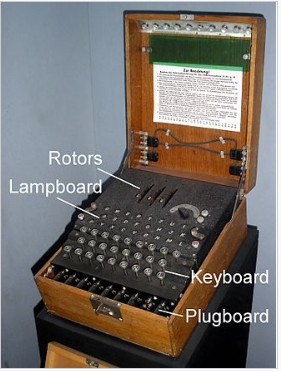
\includegraphics[width=1\linewidth]{800px-EnigmaMachineLabeled.jpg} 
    \caption{Máquina enigma con sus componentes.}
    \label{fig:wrapfig}
\end{wrapfigure}

La Máquina Enigma es un dispositivo electro-mecánico. Esencialmente, está compuesta por un teclado con distribución QWERTZ, un set de lámparas que representan los caracteres del diccionario, una serie de rotores (generalmente tres o cuatro) y un tablero de conexiones (conocido como $Plugboard$). Al presionar un botón del teclado, el caracter presionado es cifrado y el resultado puede ser observado en la lámpara asociada al caracter resultante del proceso. Asimismo, el criptograma puede ser descifrado introduciéndolo en el teclado de una máquina que tenga una configuración idéntica en sus elementos (tablero de conexiones y rotores) que la máquina que realizó el cifrado.



Las siguiente subsecciones se proponen analizar los distintos aspectos y componentes de la máquina.

\subsubsection{Flujo de corriente eléctrica}

En la siguiente figura se esquematiza cómo es el flujo de la corriente y el cableado interno dentro de la Máquina Enigma, desde que se presiona el caracter que se quiere codificar hasta que se enciende la luz que representa el caracter cifrado. 

\begin{figure}[H]
    \centering
    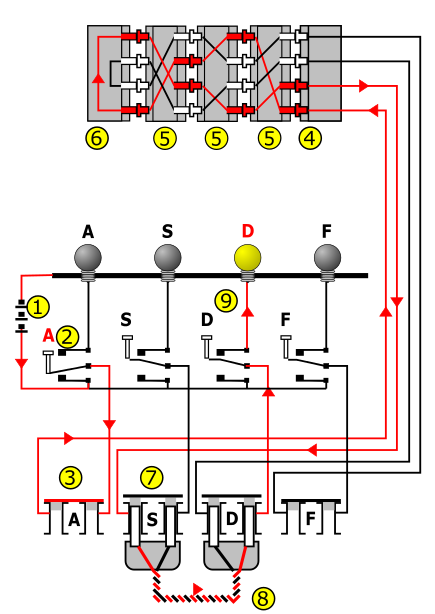
\includegraphics[scale=0.4]{current-flow.png}
    \caption{Flujo de corriente de la máquina.\cite{wikimedia3}}
    \label{fig:my_label}
\end{figure}

La corriente comienza a fluir desde la batería [1] a través del switch de la tecla presionada [2] hacia el \textit{plugboard}. El \textit{plugboard} permite cambiar un caracter por otro mediante un cableo. Una vez que pasa por el \textit{plugboard}, la corriente se dirige hacia la rueda de entrada [4] de los rotores. Para el caso de la letra A, no se realiza ningún cambio. Luego, atraviesa los rotores [5], y llega a un reflector [6], que refleja la señal para que atraviese nuevamente los rotores y la rueda de entrada, y vuelva al \textit{plugboard}. En este caso, ingresa al tablero de conexiones a través de la entrada para la letra S, pero esta sí está conectada a la letra D a través de un cable [8] por lo que la corriente fluye hacia la lámpara asociada a dicha letra y a través de un switch [9] enciende la lámpara.

\subsubsection{Rotor}

El rotor es el elemento fundamental de la Máquina Enigma. En sí mismo, un rotor no realiza más que una sustitución de un caracter por otro. Su valor agregado radica en la sustitución realizada es de caracter polialfabético: debido a su rotación constante, una letra puede ser sustituida por varias a medida que se ingresa en el teclado un mensaje que se desea encriptar. 

\begin{wrapfigure}{r}{0.3\textwidth}
    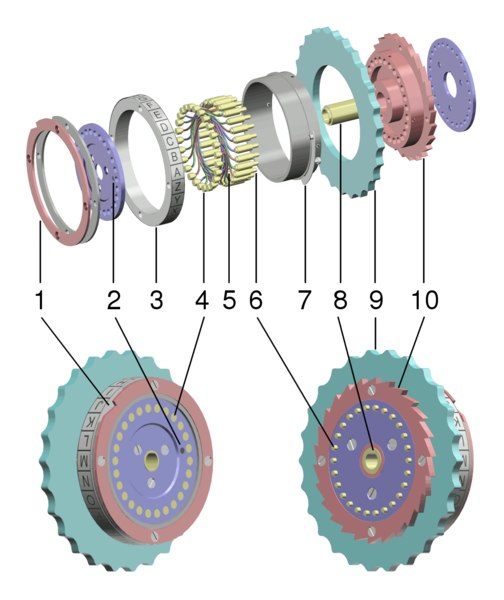
\includegraphics[width=1\linewidth]{enigma-rotor.png} 
    \caption{Rotor y sus partes.\cite{wikimedia1}}
    \label{fig:wrapfig}
\end{wrapfigure}

El rotor consiste básicamente en un disco metálico dentado [9] de aproximadamente 4 pulgadas de diámetro. En su interior, se encuentran 26 conexiones de alambre metálico [5] que conectan la entrada de 26 contactos con resorte [6] del lado derecho a 26 contactos planos en el lado izquierdo [4], estructura que se sostiene mediante un eje hueco [8] que atraviesa el interior. En el exterior se halla un anillo [3] con 26 letras o números y un $notch$, que consiste en una pequeña muesca posicionada en alguna de las letras. Este anillo puede rotar alrededor del disco y se traba en alguna posición mediante un arco con resorte[7]. Un cambio en la posición del anillo generará un cambio en la posición del \textit{notch} y del alfabeto, relativo al cableo interno del rotor (es decir, agregará un \textit{offset} a la codificación que realice el rotor). La  configuración de la posición del anillo es conocida como \textit{Ringstellung} y su posición puede ser apreciada mediante una marca[2]. Por último, cada rotor posee en su sección izquierda al \textit{notch} y en su sección derecha un trinquete[10]. Estos componentes son los que se combinan junto al mecanismo de avance para realizar una rotación.

\begin{figure}[h]

\begin{subfigure}{0.5\textwidth}
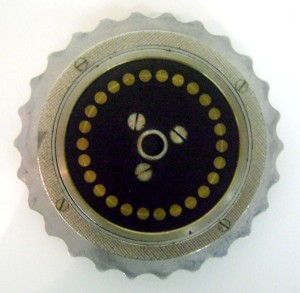
\includegraphics[width=1\linewidth]{rotor-view-left.jpg} 
\caption{Vista izquierda del rotor con su único $notch$.}
\label{fig:subim1}
\end{subfigure}
\begin{subfigure}{0.5\textwidth}
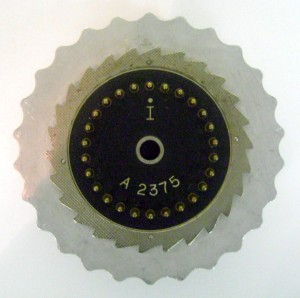
\includegraphics[width=0.97\linewidth]{rotor-view-right.jpg}
\caption{Vista derecha del rotor con su trinquete dentado.}
\label{fig:subim2}
\end{subfigure}

\caption{Vistas laterales del rotor.\cite{rijmenants}}
\label{fig:image2}
\end{figure}

Originalmente, la máquina que utilizaban la Armada y la Fuerza Aérea alemana poseía tres rotores. Luego, en 1938, la cantidad fue extendida a cinco rotores (cada uno con un \textit{notch}, y se les asignaron los números romanos I, II, III, IV, V para distinguirlos. Más tarde, al set se agregaron los rotores VI, VII, VII, cuya particularidad era que tenían dos \textit{notches} cada uno. 

El cableo interno del rotor y su rotación son quienes realizan el encriptado. Cada uno de los rotores tiene su propia tabla de cifrado, la cual representa las conexiones que existen entre los pins de entrada en el lado derecho y los pins de salida del lado izquierdo. Por ejemplo, para los primeros cinco rotores, los cuáles poseen únicamente un $notch$, sus tablas son las siguientes:

\begin{figure}[H]
    \centering
    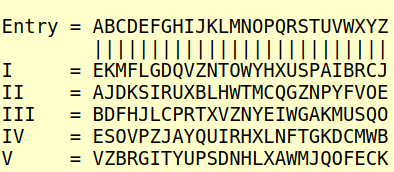
\includegraphics[scale=0.38]{tabla-rotor.png}
    \caption{Tabla de cableo interno de rotores I a V.\cite{rijmenants}}
    \label{fig:my_label}
\end{figure}

Es importante tener en cuenta que este \textit{mapping} entre letras no necesariamente (de hecho, rara vez sucederá) significa que una señal para la letra A proveniente del \textit{plugboard} termine codificada como una E (si analizamos el rotor I). El resultado final dependerá además de la posición en la que se encuentre el rotor al momento en el que ingresa la señal (podría ingresar por cualquiera de los pines), además del \textit{Ringstellung} que agregará un \textit{offset} a la salida.

Para realizar el encriptado de una señal correspondiente a un caracter proveniente del \textit{plugboard}, se sigue el siguiente proceso. Cuando una tecla es presionada, los rotores avanzan antes de que la señal eléctrica los atraviese. A cotinuación, se procederá a ilustrar el proceso de encriptado mediante un ejemplo que utiliza al Rotor I. El anillo se corresponde con las letras encerradas en el campo gris; el cableo interno está encerrado por las dos columnas de letras encerradas en el campo blanco; la posición del rotor está indicada por la letra enmarcada en negro que se encuentra en el anillo exterior; la configuración del anillo o \textit{Ringstellung} se indica con una pequeña marca negra al lado derecho de alguna letra del anillo gris; y por último los alfabetos que se encuentran a la derecha e izquierda del rotor representan los pines de entrada y salida respectivamente. Se considera la siguiente imagen:

\begin{figure}[H]
    \centering
    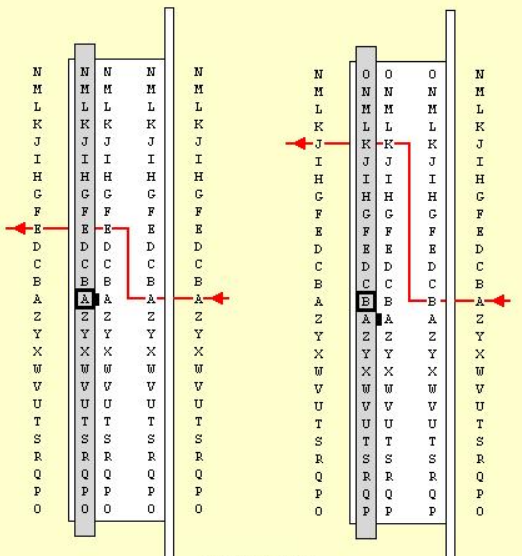
\includegraphics[scale=0.4]{rotor-ejs-1.png}
    \caption{Cifrado seguido de la letra A en el Rotor I.\cite{rijmenants}}
    \label{fig:my_label}
\end{figure}

La imagen de la izquierda muestra como se realiza el cifrado en el Rotor I cuando la letra A se presiona dos veces consecutivas. Nótese que la configuración del anillo del rotor es A-01, y la posición del rotor también es A. La señal de la letra A, proveniente del \textit{plugboard}, arriba a la posición A e ingresa por el pin A, atraviesa el cableado interno pasando de la A a la E, y atraviesa el anillo para terminar saliendo por el pin E.
Por su lado, en la imagen de la derecha, el rotor ha avanzado a la posición B. La señal arriba a la posición A, pero ahora ingresa por el pin B para ser redirigida al caracter K. Sin embargo, como todo el rotor ha avanzado una posición, la señal termina saliendo por la posición J hacia el rotor siguiente.
Para este ejemplo no se ha tenido en cuenta una configuración del anillo que agregue un \textit{offset} al cifrado resultante. Consideremos los siguientes dos ejemplos: 

\begin{figure}[H]
    \centering
    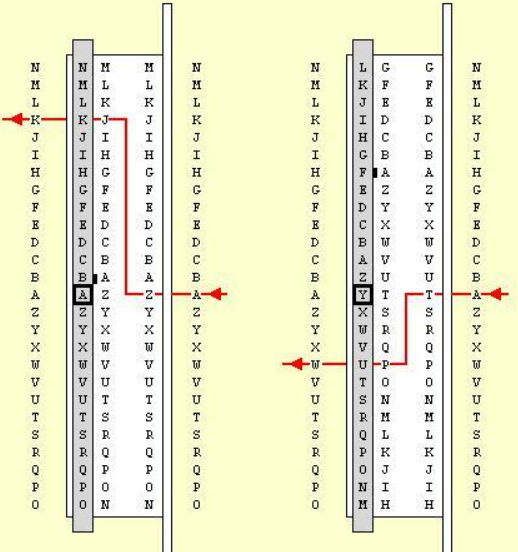
\includegraphics[scale=0.4]{rotor-ejs-2.png}
    \caption{Cifrado de la letra A en el Rotor I con distintos \textit{Ringstellung}.\cite{rijmenants}}
    \label{fig:my_label}
\end{figure}

En la imagen de la izquierda, la configuración del anillo es B-02. Como la posición del rotor es A, parecería ser que al ingresar por la posición A el cableado interno sería A $\rightarrow$ E. Sin embargo, el \textit{Ringstellung} agrega un \textit{offset} al cableado y la señal ingresa por el pin Z y es redirigida al pin J. A su vez, el pin de salida J no coincide con la posición J ya que este \textit{offset} también afecta a los contactos de la salida, por lo tanto la señal finaliza saliendo por la posición K hacia el siguiente rotor. 

La imagen de la derecha es el caso más complejo a analizar. En este caso, la configuración del anillo es F-06, y la posición del rotor es Y. La tecla presionada es nuevamente la A, y el pin de entrada al centro del rotor resulta ser la posición del rotor desplazada alfabéticamente en seis posiciones, es decir la letra T. Luego, el cableo interno del Rotor I redirige la señal hacia el pin P, que coincide con la posición U del anillo. Finalmente, como nos encontramos en la posición Y del rotor, la señal termina saliendo por la posición W hacia el rotor siguiente. Nótese que la salida está desplazada en siete posiciones alfabéticas: cinco entre la A y la F por la configuración del anillo, y dos adicionales entre la Y y la A. 

\subsubsection{Mecanismo de avance}

Cada vez que se presiona una tecla, se modifica la posición de al menos uno de los rotores de la máquina. Esto significa que se obtendrán cifrados diferentes cuando se presione la misma tecla en forma consecutiva. Aquí, en parte, radica el poder para encriptar la máquina: existen un número enorme de posibilidades de configuración y posicionamiento de los rotores que generan resultados distintos.
El primero de los rotores avanza siempre que se presiona una tecla. El segundo, en cambio, avanza una vez por cada 26 avances del primer rotor, es decir cada 26 teclas presionadas. El tercero, el más lento de todos, avanza una vez por cada avance del segundo rotor, es decir una vez cada 676 teclas presionadas.


\begin{figure}[H]
    \centering
    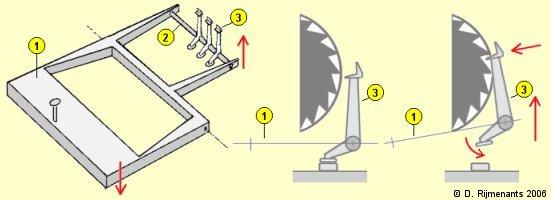
\includegraphics[scale=2]{stepping-mech.jpg}
    \caption{Mecanismo de avance de los rotores.\cite{rijmenants}}
    \label{fig:my_label}
\end{figure}

Al presionar una tecla, la barra de avance [1] se moverá hacia abajo y el eje del trinquete [2] y sus tres trinquetes [3] (uno por cada rotor) hacia arriba. Cada uno de estos tres trinquetes, que se mueven al unísono, intentará encastrarse con los dientes que recubren al rotor, para así generar un desplazamiento en el mismo. Por la forma en la que están dispuestos los rotores, solamente se podrá desplazar un rotor si el rotor de su derecha se encuentra en su posición \textit{notch}, ya que en cualquier otro caso el anillo que recubre al \textit{notch} impedirá la combinación entre el trinquete y los dientes del rotor. En el caso del rotor que se encuentra más a la derecha, ante la ausencia de un anillo que le impida accionar sobre los dientes del rotor, el trinquete siempre logrará moverlo y es por esto que el primero de los rotores avanza cada una de las veces que se ingresa una letra. 

Con la descripción realizada, podría parecer que el sistema de rotores se comporta como un odómetro. Pero adicionalmente al movimiento producido en el caso en el que el rotor de la derecha se encuentre en la posición \textit{notch}, existe una situación en la que un rotor que no es el de la derecha puede desplazarse dos veces seguidas. Esta situación sucede cuando, en el momento en el que un rotor debe avanzar porque el rotor de su derecha se encuentra en su posición \textit{notch}, este también se encuentra en su posición de \textit{turnover}. En este caso, el rotor avanzará dos veces consecutivas, en vez de esperar por un giro alfabético completo del rotor de su derecha.   

\subsubsection{Reflector}

A diferencia del rotor, en donde una letra puede ser transformada en cualquier otra dependiendo de la posición y la configuración del anillo, el reflector posee conecciones de a pares. Esto significa que si la letra G está cableada a la letra P, entonces P también lo estara a G. Si bien la tarea del reflector es simple, le agrega un grado de complejidad mayor al encriptado de un mensaje, ya que además de realizar la sustitución asociada al cableado, genera que la señal vuelva a atravesar los rotores por segunda vez en sentido contrario.

\begin{figure}[H]
    \centering
    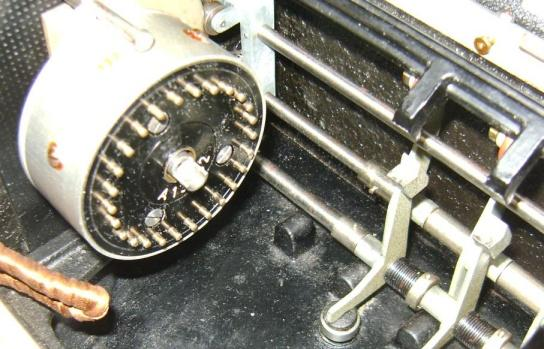
\includegraphics[scale=0.3]{reflector.jpg}
    \caption{Reflector de la Máquina Enigma.\cite{rijmenants}}
    \label{fig:my_label}
\end{figure}

\subsubsection{Plugboard}

\begin{wrapfigure}{L}{0.4\textwidth}
    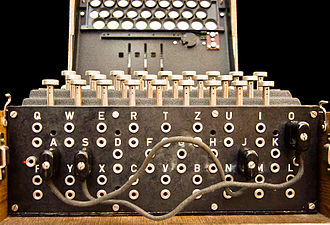
\includegraphics[width=1\linewidth]{plugboard.jpg} 
    \caption{Plugboard de la Máquina Enigma.\cite{wikimedia2}}
    \label{fig:wrapfig}
\end{wrapfigure}


El \textit{plugboard} se encuentra al frente de la máquina. Como se ha analizado previamente, la señal atraviesa el \textit{plugboard} antes de llegar a la entrada del sistema de rotores y antes de finalizar su recorrido en el set de lámparas. Su función básica es la de realizar una sustitución simple entre letras antes de que la señal llegue al correspondiente destino. Su caracterísitica más importante es que la configuración puede ser modificada por el operador que va a utilizar la máquina, generando así un montón de combinaciones posibles y reforzando la seguridad criptográfica del criptograma final. La sustitución es entre pares: si por ejemplo se conectan las entradas U y J, toda señal que entre por la letra U será cambiada por una J y viceversa.

\subsection{Espacio de claves}

El espacio de claves de la Máquina Enigma está compuesto por todas las combinaciones posibles de los componentes configurables. En primer lugar, encontramos las posibles permutaciones del \textit{plugboard}: se deben tener en cuenta todas permutaciones posibles de pares de letras que se pueden realizar. En segundo lugar, se debe considerar el armado del sistema de rotores: se debe recordar que los alemanes utilizaban varios rotores distintos, y que el orden de los mismos dentro de la máquina podía variar. Por último, se deben contemplar los aspectos configurables de cada rotor: además de su cableo interno según la elección del tipo de rotor, se deben tener en cuenta la configuración de su anillo y su posición inicial. 

En el caso de la máquina con tres rotores, existen $26^3=17576$ configuraciones distintas para las posiciones iniciales de los rotores. Por otro lado, considerando que inicialmente poseían 5 rotores distintos, existen $5*4*3=60$ combinaciones para colocar los rotores en la máquina. Por otro lado cada rotor puede configurar la posición del anillo por lo que esto agrega $26^3$ posibilidades. Finalmente, el \textit{plugboard} provee la mayor posibilidad de armar configuraciones distintas. Se considerará la utilización de diez cables, número que solían utilizar los alemanes. La fórmula matemática que nos permite conocer cuántas combinaciones posibles existen para $n$ cables es:

\begin{equation}
    |\omega| = \frac{26!}{(26 - 2n)! \cdot n! \cdot 2^n}
\end{equation}

Esto nos da 150738274937250 combinaciones posibles para el $plugboard$.

Finalmente, realizando las cuentas correspodientes, llegamos a que el espacio de claves de la máquina es de: 

\begin{equation}
    60*17576*17576*150738274937250 = 2793925870508516103360000
\end{equation}
Para comparar con largos que generan algoritmos de clave simétrica modernos, es posible formular ese número en potencia de dos, lo que nos da un resultado de aproximadamente $2^{81,20\ldots}$ posibilidades. Debe aclararse que la cuenta realizada considera el uso en la práctica de la Máquina Enigma. Está claro que, teóricamente, el espacio de claves es abrumadoramente mayor, ya que deberían considerarse los cableos internos de cada rotor y la posibilidad de utilizar una cantidad arbitraria de cables en vez de diez en el \textit{plugboard}.

\subsection{Uso de modelos de lenguaje}

\subsubsection{Motivación}

Un modelo de lenguaje $M$ es tal que contiene caracteristicas únicas del idioma en cuestión, (en nuestro caso particular, entrenamos utilizando libros de dominio público en idioma inglés) sobre el cual se puede computar alguna función de pérdida $loss_M$ para, dado un criptograma con cada clave $K_i$, explorar cada texto plano $t_{K_i}$ buscando:

\begin{align}
    \argmin_{K_i} {loss}_M(t_{K_i})
\end{align}

Dado que, como se mostrará posteriormente, el espacio de claves posee cierta redundancia y además se puede explorar por medio de un gradiente, no necesitaremos explorar todas las claves $K_i$.

\subsubsection{Divergencia de Kullback-Leibler}

La divergencia de \textit{Kullback-Leibler} es una medida de similitud entre dos funciones de distribución probabilística. Siendo $P$ y $Q$ las funciones de distribución probabilística, se puede calcular cómo:

\begin{equation}
    D_{KL}(P||Q) =  \sum_{i} P(i) \cdot ln \frac{P(i)}{Q(i)} 
\end{equation}

Algunas propiedades de esta medida son:

\begin{itemize}
    \item Es siempre positiva.
    \item Es nula solamente en el caso en el que $P = Q$.
    \item No es simétrica (no se trata de una medida de distancia).
\end{itemize}

Esta divergencia será utilizada en algunos de nuestros modelos como función de pérdida.

\subsubsection{Index of Coincidence o índice de coincidencia\cite{ic}}

Sea $n_i$ la frecuencia de cada letra $c$ del alfabeto considerando un texto de largo $N$. Se puede calcular el índice de coincidencia IC como:

\begin{align}
    {IC} = \frac{\sum_{i=1}^{|c|} n_i(n_i-1)}{N(N-1)/c}
\end{align}

Cada idioma tiene su indíce de coincidencia característico. Esta cantidad nos habla de cómo es la forma de la distribución de probabilidad sobre los caracteres. A su vez, una cualidad importante de esta medida es que es resiliente a permutaciones. Por ejemplo, si se realiza un intercambio de la letra A por la P y viceversa, entonces ahora $n_A$ tendrá el valor que antes tenía $n_P$ y viceversa, y el cálculo daría lo mismo.

\subsubsection{Modelo de frecuencias por caracter}

El primer modelo implementado consiste simplemente en contar la frecuencia de caracteres del idioma en cuestión y compararlo con el texto recuperado $t_k$ con dos versiones de distintas funciones de pérdida.

La primera, implementando el índice de coincidencia, es:

\begin{align}
    {loss_M}(t_k) = |{IC}_{idioma} - \frac{\sum_{i=1}^{|c|} n_i(n_i-1)}{N(N-1)/c}|
\end{align}

La segunda versión utilizan la divergencia de Kullback-Leibler (2) entre la distribución de caracteres del idioma y de $t_k$.

El uso del índice de coincidencia (el utilizado en el paper original) es más robusto ante permutaciones pero, por otro lado, si se tomara el texto original y se aplicaran 13 permutaciones cualesquiera a las letras, este índice nos indicaría la misma cantidad para el texto sin permutar y para el que recibió las permutaciones. Por otro lado, la divergencia de KL exige que la proporción de cada caracter en el texto recuperado sea la que corresponde para ese mismo caracter en el modelo del lenguaje, por lo que cualquier permutación aumentará el error y menos textos colisionarán con la misma pérdida, aumentando la \textit{especificidad} pero perdiendo \textit{exhaustividad}.

\subsubsection{Cadena de Markov de orden 1}

En las cadenas de Markov también se modela la probabilidad de los caracteres, pero condicionados al caracter anterior, por lo que se tendrán distribuciones $P(c_j)_{|c_i}$ donde para cada caracter $c_j$ existirá una probabilidad distinta dado el caracter anterior $c_i$. A su vez, cada caracter $c_i$ tiene una probabilidad a priori $P(c_i)$. La pérdida para este modelo de lenguaje se calcula como la divergencia de KL para cada distribución condicionada, ponderada por la probabilidad a priori del caracter que condiciona. Considerando $P$ a las probabilidades sobre el modelo de lenguaje y $Q$ a las probabilidades sobre el texto recuperado, la función de pérdida queda:

\begin{align}
    {loss_M}(t_k) = \sum_{i=1}^{|c|} P(c_i) D_{KL}(P_{|c_i}||Q_{|c_i})
\end{align}

Como con la divergencia de KL descripta para el modelo de lenguaje de caracteres, nuevamente se le piden más condiciones a $t_k$ para coincidir con la función de pérdida, por lo que se espera que esta métrica sea más excluyente.

\section{Experimentación y resultados}

\subsection{Evaluación de los modelos de lenguaje}

A partir de los modelos de lenguaje introducidos en el marco teórico, se buscó determinar la posibilidad de reproducir la investigación de Gillogly utilizando no solamente el \textit{Index of Coincidence}, sino también el modelo de lenguaje basado en frecuencias por caracter y el modelo de cadenas de Markov de largo uno.

Para esto, fueron implementados los tres modelos de lenguaje, con el fin de compararlos y evaluar su performance variando el largo de la cadena a desencriptar. La Máquina Enigma utilizada para encriptar y desencriptar se armó tomando un orden de rotores aleatorio, sin agregarles offset y sin permutaciones en el plugboard. Luego, se obtuvo un listado de textos encriptados, cada uno con un largo distinto. A continuación, se procedió a desencriptar los criptogramas utilizando distintas configuraciones de rotores (explorando el espacio de claves), y se elaboró un ranking ordenado de menor a mayor según el resultado de evaluar la función de pérdida según un modelo del lenguaje al texto desencriptado. Finalmente, en este ranking, se buscó la posición de la clave original que había sido encriptada, evaluando de esta forma la robustez de los modelos. Lógicamente, se esperaba ver más dificultad (una posición mayor en el ranking) en textos cortos.

\begin{figure}[H]
    \centering
    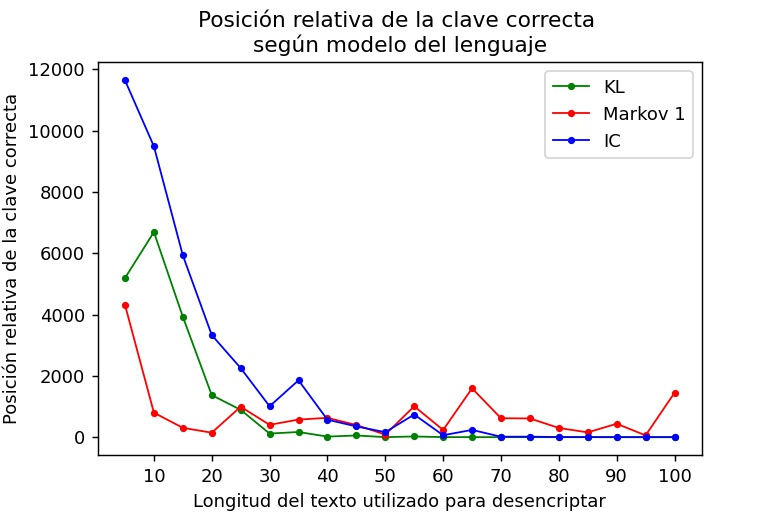
\includegraphics[scale=0.8]{language_model_length.jpg}
    \caption{Posición relativa de la clave correcta según modelo y largo del texto}
    \label{fig:my_label}
\end{figure}

De esta forma, se pudo validar que los modelos incorporados parecen ser más robustos en algunos casos en los cuales el IC no lo es, ya que como fue explicado en las secciones previas, los modelos agregados son más restrictivos.

\subsection{Implementación de Gillogly (1995)\cite{gillogly}}

Se realizó una implementación (con algunos cambios) del algoritmo implementado en el paper original, incorporando los 3 modelos de lenguaje previamente descriptos. Al igual que en el paper original, se acotó la búsqueda de claves a explorar tomando 3 de los 5 rotores y el mismo reflector. Utilizar más tipos de rotores u otros reflectores solo implicaría explorar más permutaciones, cada una combinada con cada reflector.

Los pasos del algoritmo implementado son:

\begin{enumerate}
  \item A partir de un criptograma, se exploran las 60 permutaciones de 3 rotores tomados de a 5 para sus $26^3$ claves posibles con los $Ringstellung$ en 'A' y sin conexiones en el plugboard. Para cada configuración, se calcula la función de pérdida del resultado desencriptado. Este paso es el más costoso.
  \item Para las 6 mejores configuraciones de rotores y claves del paso anterior según cada una de las 3 funciones de pérdida (18 en total), se exploran las $26^3$ combinaciones posibles del $Ringstellung$, también calculando la función de pérdida.
  \item Se toman las 10 mejores combinaciones de rotores, claves y $Ringstellung$ para cada una de las pérdidas de los modelos de lenguaje (30 en total) y se procede a realizar la búsqueda del plugboard (conociendo el tamaño del plugboard original) de una forma tal que se corresponde con un descenso por el gradiente. Se agrega el mejor 'cable' posible al plugboard, y luego sobre esa solución se vuelve a agregar otro, y así sucesivamente hasta converger a la mejor solución.
\end{enumerate}

Esta implementación difiere ligeramente de la utilizada en el paper original. En dicho paper, en lugar de explorar todo el $Ringstellung$, se explora la configuración de los rotores utilizando descenso por el gradiente, primero para rotor rapido y, al encontrar la mejor configuración para este, se lo mantiene fijo y se busca la mejor configuracón para el segundo. No se realiza una búsqueda para el tercero (porque, según dice el autor de la investigación, esto no afecta al resultado de salida). En la implementación realizada se decidió explorar todo el espacio de claves ya que no era muy costoso ($\frac{1}{60}$ parte del costo del primer paso).

Como explicamos en la sección 2.2 de espacio de claves, la mayor parte del espacio está conformado por el plugboard. Esta sección del espacio es aquella donde más se notará la capacidad de descender paso a paso por la clave y por lo tanto, más alla de la abrumadora combinatoria, será la que menos costos computacionales insumirá para el algoritmo.

\subsection{Ejemplo}

En muchos ejemplos pudimos apreciar la redundancia del espacio de claves. Uno de ellos fue cifrando el siguiente fragmento del texto \textit{Pride and prejudice}:
\begin{small}
\begin{Verbatim}
NCEPUTMYFOOTOUTOFDOORSTHOUGHIWASTHEREAFORTNIGHTNOTONEPARTYORSCHEMEORANYTHING
TOBESURELONDONWASRATHERTHINBUTHOWEVERTHELITTLETHEATREWASOPENWELLANDSOJUSTAST
HECARRIAGECAMETOTHEDOORMYUNCLEWASCALLEDAWAYUPONBUSINESSTOTHATHORRIDMANMRSTON
EANDTHENYOUKNOWWHENONCETHEYGETTOGETHERTHEREISNOENDOFITWELLIWASSOFRIGHTENEDID
IDNOTKNOWWHATTODOFORMYUNCLEWASTOGIVEMEAWAYANDIFWEWEREBEYONDTHEHOURWECOULDNOT
BEMARRIEDALLDAYBUTLUCKILYHECAMEBACKAGAININTENMINUTESTIMEANDTHENWEALLSETOUTHO
WEVERIRECOLLECTEDAFTERWARDSTHATIFHEHADBEENPREVENTEDGOINGTHEWEDDINGNEEDNOTBEP
UTOFFFORMRDARCYMIGHTHAVEDONEASWELLMRDARCYREPEATEDELIZABETHINUTTERAMAZEMENTOH
YESHEWASTOCOMETHEREWITHWICKHAMYOUKNOWBUTGRACIOUSMEIQUITEFORGOTIOUGHTNOTTOHAV
ESAIDAWORDABOUTITIPROMISEDTHEMSOFAITHFULLYWHATWILLWICKHAMSAYITWASTOBESUCHASE
CRETIFITWASTOBESECRETSAIDJANESAYNOTANOTHERWORDONTHESUBJECTYOUMAYDEPENDUPONMY
SEEKINGNOFURTHEROHCERTAINLYSAIDELIZABETHTHOUGHBURNINGWITHCURIOSITYWEWILLASKY
OUNOQUESTIONSTHANKYOUSAIDLYDIAFORIFYOUDIDISHOULDCERTAINLYTELLYOUALLANDTHENWI
CKHAMWOULDBE
\end{Verbatim}
\end{small}

El criptograma se obtuvo a partir de la siguiente configuración de rotores, de derecha a izquierda:

\begin{itemize}
  \item Rotor II con offset 8 y $Ringstellung$ 20.
  \item Rotor IV con offset 22 y $Ringstellung$ 3.
  \item Rotor V con offset 7 y $Ringstellung$ 2.
\end{itemize}

Y permutaciones del plugboard: $CD$, $GU$ y $ZW$.

Luego de haber ejecutado el primer paso del algoritmo sobre ese criptograma, la distribución de los scores ($-{loss}$) es la siguiente para los tres modelos:

\begin{figure}[!htb]
\minipage{0.32\textwidth}
  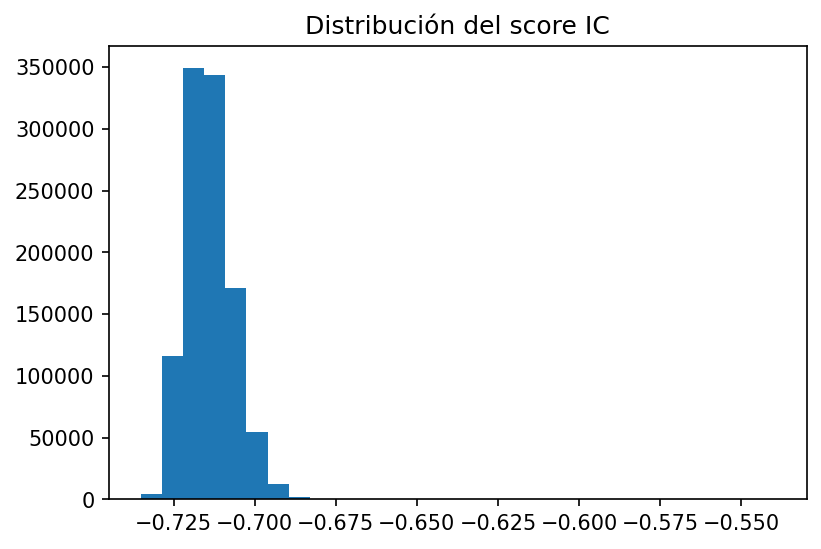
\includegraphics[width=\linewidth]{ic.png}
  \caption{Distribución del score de IC para los $t_k$}
\endminipage\hfill
\minipage{0.32\textwidth}
  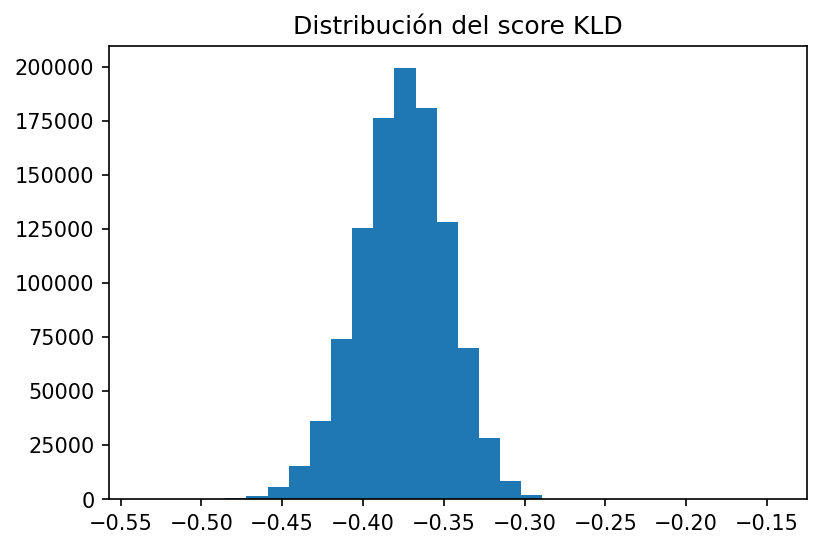
\includegraphics[width=\linewidth]{kld.png}
  \caption{Distribución del score KLD para los $t_k$}
\endminipage\hfill
\minipage{0.32\textwidth}%
  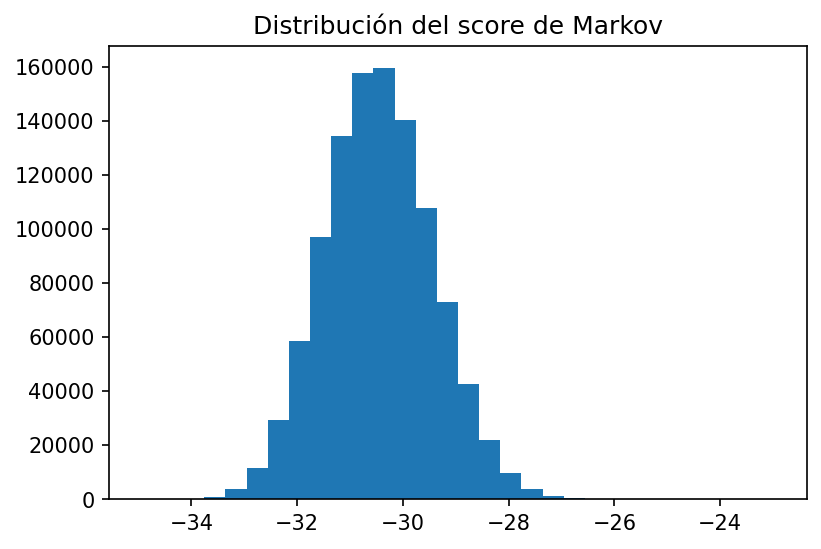
\includegraphics[width=\linewidth]{markov.png}
  \caption{Distribución del score de Markov para los $t_k$}
\endminipage
\end{figure}

Los 3 modelos del lenguaje coinciden en que la mejor configuración (mayor score) es, derecha a izquierda:

\begin{itemize}
  \item Rotor II con offset 14 y $Ringstellung$ 0.
  \item Rotor IV con offset 19 y $Ringstellung$ 0.
  \item Rotor V con offset 5 y $Ringstellung$ 0.
\end{itemize}

En el paso 2 se exploran todas las $Ringstellung$, y los tres modelos vuelven a coincidir:

\begin{itemize}
  \item Rotor II con offset 14 y $Ringstellung$ 0
  \item Rotor IV con offset 19 y $Ringstellung$ 0
  \item Rotor V con offset 5 y $Ringstellung$ 0
\end{itemize}

Finalmente en el último paso se busca el plugboard y, nuevamente, la solución de menor error para los 3 modelos es la anterior con el mismo plugboard utilizado para encriptar: $CD$, $GU$ y $ZW$. 
Nótese que la clave final encontrada es distinta a la original, pero que sin embargo se recuperaron 733 caracteres de los 1000 caracteres originales. Este es un claro ejemplo de la redundancia en el espacio.

He aquí el mensaje recuperado con aquellos caracteres que no coinciden con el original remarcados en rojo. También, se puede apreciar que los errores tienen una periodicidad:

\begin{small}
\begin{Verbatim}[commandchars=\\\{\}]
NCEPUTMYFOOTOUTO\textcolor{red}{IUBAJX}THOUGHIWASTHEREAFORT\textcolor{red}{GULCZ}NOTONEPARTYORSCHEMEOR\textcolor{red}{WLSOSL}NGT
OBESURELONDONWASR\textcolor{red}{FRLUSM}HINBUTHOWEVERTHELITT\textcolor{red}{UZIWCN}TREWASOPENWELLANDSOJ\textcolor{red}{XWVZUS}HE
CARRIAGECAMETOTHED\textcolor{red}{INUWSN}NCLEWASCALLEDAWAYUPO\textcolor{red}{GINFCA}ESSTOTHATHORRIDMANMR\textcolor{red}{FQGQGG}N
DTHENYOUKNOWWHENONC\textcolor{red}{DKYMJP}ETTOGETHERTHEREISNOE\textcolor{red}{ZQKSXD}WELLIWASSOFRIGHTENED\textcolor{red}{EZKZVJ}
\textcolor{red}{}TKNOWWHATTODOFORMYUN\textcolor{red}{DPLNMT}TOGIVEMEAWAYANDIFWEW\textcolor{red}{OVCZHNXMUOOBSNAVGHYWXMKVZXUQRRG}
\textcolor{red}{IMBBCMORTKPXYZLSHFIJDLWQDPOFIAEZESFTTKKDHNAIJNZOZSFNL}DTHENWEALLSETOUTHOWE\textcolor{red}{GTYZ}
\textcolor{red}{UL}COLLECTEDAFTERWARDST\textcolor{red}{Z}A\textcolor{red}{GCAW}EHADBEENPREVENTEDGOI\textcolor{red}{IBBE}E\textcolor{red}{M}EDDINGNEEDNOTBEPUTOF\textcolor{red}{WU}O
\textcolor{red}{IE}RDARCYMIGHTHAVEDONEAS\textcolor{red}{BRIADN}DARCYREPEATEDELIZABE\textcolor{red}{POSVJI}TERAMAZEMENTOHYESHEW\textcolor{red}{DV}
\textcolor{red}{QTDD}METHEREWITHWICKHAMYO\textcolor{red}{QDMTBA}UTGRACIOUSMEIQUITEFO\textcolor{red}{YNZPWR}UGHTNOTTOHAVESAIDAWO\textcolor{red}{O}
\textcolor{red}{TGLEQ}TITIPROMISEDTHEMSOFA\textcolor{red}{SP}H\textcolor{red}{EOQ}LYWHATWILLWICKHAMSAYI\textcolor{red}{ZA}A\textcolor{red}{VC}OBESUCHASECRETIFITWA
S\textcolor{red}{SGYMC}ECRETSAIDJANESAYNOTA\textcolor{red}{BUDW}ERWORDONTHESUBJECTYOUM\textcolor{red}{XEA}E\textcolor{red}{SU}NDUPONMYSEEKINGNOFU
R\textcolor{red}{UK}ER\textcolor{red}{P}HCERTAINLYSAIDELIZABE\textcolor{red}{XBDGBW}GHBURNINGWITHCURIOSI\textcolor{red}{PBLIXP}LLASKYOUNOQUESTION
ST\textcolor{red}{LEZFPS}USAIDLYDIAFORIFYOUDI\textcolor{red}{VGXJNP}LDCERTAINLYTELLYOUAL\textcolor{red}{WHTYKF}ENWICKHAMWOULDBE
\end{Verbatim}
\end{small}

\subsection{Resultados}

En total, se realizaron 100 corridas, dividiéndolas de a 20 para cantidades distintas de permutaciones (tamaño del plugboard) en el plugboard (1,3,5,7 y 9). Para generar los criptogramas fueron utilizados textos planos de 1000 caracteres aleatorios tomados de \textit{Pride and Prejudice}, y los modelos del lenguaje fueron entrenados con \textit{Alices Adventures in Wonderland}.

La efectividad del método (definido como en el paper original, es decir que se considera una corrida como exitosa cuando se recupera más del 80\% del texto original) en función del tamaño del plugboard es la siguiente:

\begin{figure}[H]
    \centering
    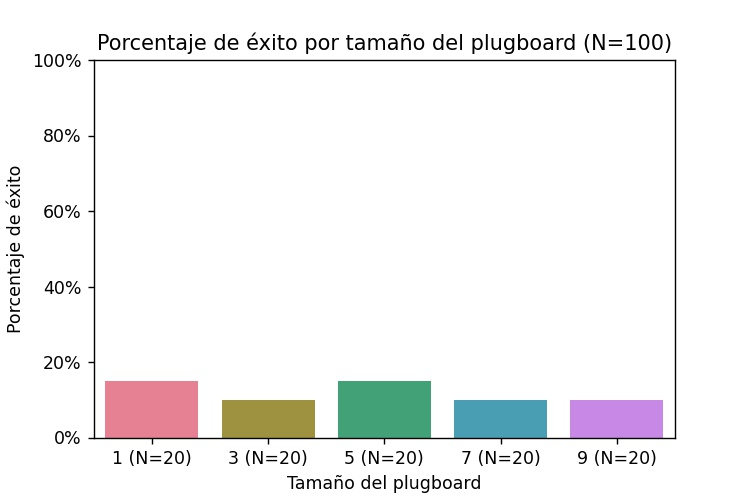
\includegraphics[scale=0.8]{success.jpg}
    \caption{Porcentaje de éxito por tamaño del plugboard}
    \label{fig:my_label}
\end{figure}

Los resultados obtenidos difieren del paper original: la tasa de éxito obtenida por nuestra implementación es menor en plugboards mas chicos y mayor en plugboards más grandes.

La corrida con error más grande y más pequeño obtenido en función del tamaño del plugboard puede verse a continuación:

\begin{figure}[H]
    \centering
    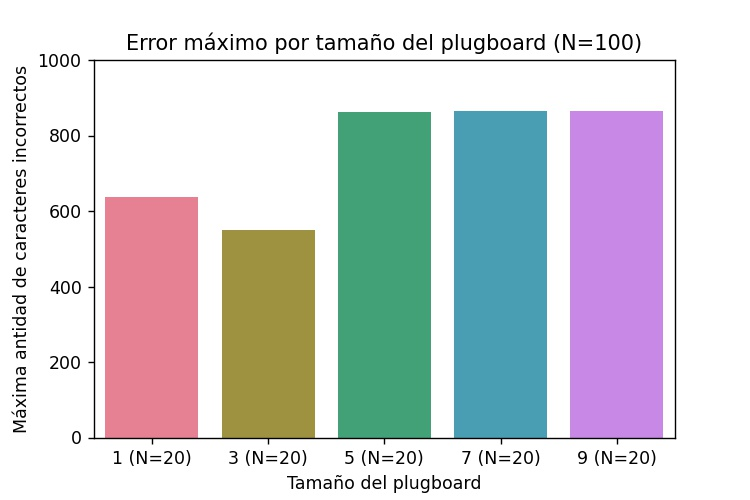
\includegraphics[scale=0.8]{max_error.jpg}
    \caption{Mayor error en función del tamaño del plugboard}
    \label{fig:my_label}
\end{figure}

\begin{figure}[H]
    \centering
    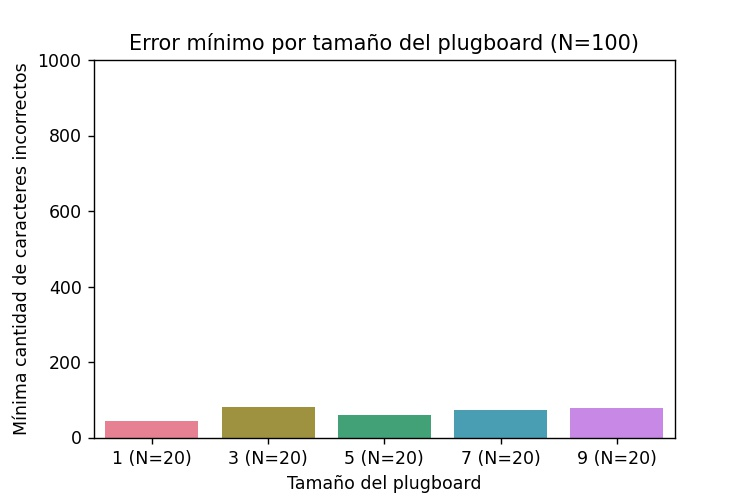
\includegraphics[scale=0.8]{min_error.jpg}
    \caption{Menor error en función del tamaño del plugboard}
    \label{fig:my_label}
\end{figure}

Mientras que la distribución del error según el tamaño del plugboard puede apreciarse en el siguiente gráfico:

\begin{figure}[H]
    \centering
    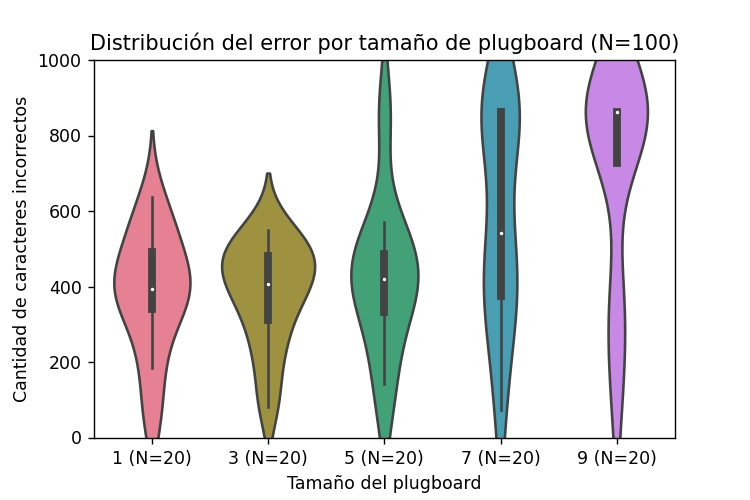
\includegraphics[scale=0.8]{error_dist.jpg}
    \caption{Distribución del error en función del tamaño del plugboard}
    \label{fig:my_label}
\end{figure}

Sin embargo, si consideramos como éxito encontrar al final de una corrida el plugboard correcto o los rotores (sin considerar su offset y \textit{ringstellung}) correctos en el orden correcto, las tasas de éxito para estos distintos casos son:

\begin{figure}[H]
    \centering
    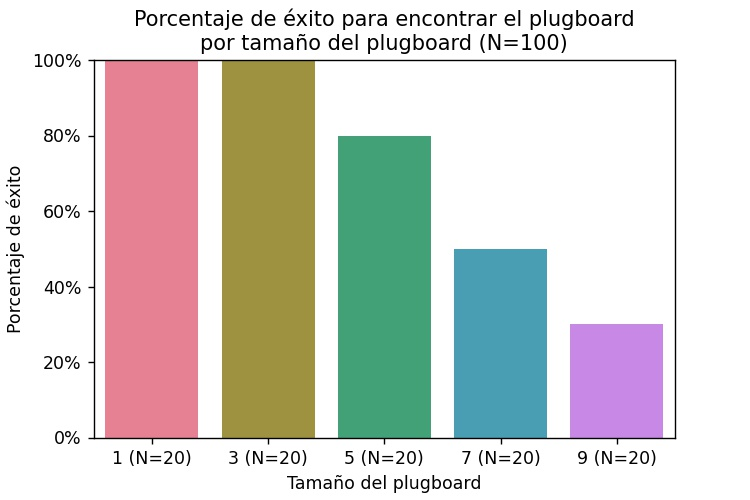
\includegraphics[scale=0.8]{plugboard_success.jpg}
    \caption{Porcentaje de éxito para encontrar el plugboard en función del tamaño del plugboard}
    \label{fig:my_label}
\end{figure}

\begin{figure}[H]
    \centering
    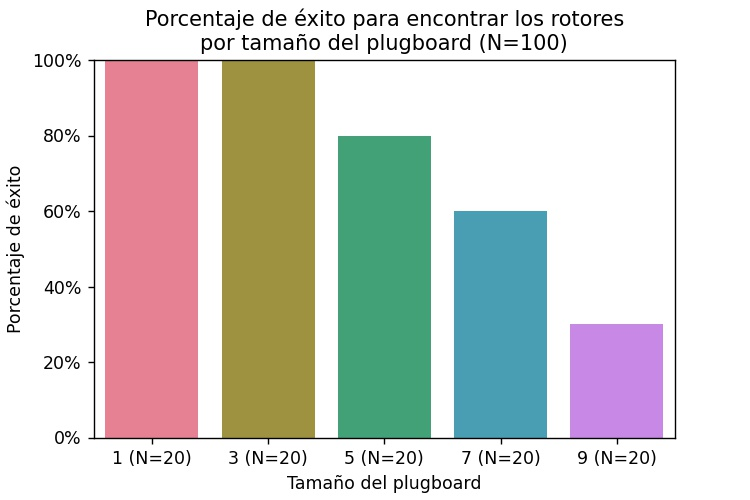
\includegraphics[scale=0.8]{rotor_order_success.jpg}
    \caption{Porcentaje de éxito para encontrar los rotores en función del tamaño del plugboard}
    \label{fig:my_label}
\end{figure}

Esto nos sugiere que si volvemos a correr el algoritmo pero fijando o bien los rotores, o bien el plugboard, o ambas, podremos achicar el espacio de búsqueda y encontrar una mejor solución.

\subsubsection{Coincidencias con la implementación original}

\begin{itemize}
  \item Es posible atacar el cifrado de la Máquina Enigma solo con el texto cifrado.
  \item Es más facil realizar el ataque si el plugboard utilizado es más chico (menos permutaciones).
  \item La mayoría del espacio de claves (plugboard) puede explorarse utilizando descenso por el gradiente.
\end{itemize}

\subsubsection{Diferencias con la implementación original}
\begin{itemize}
  \item No se aprecia mucha diferencia en el porcentaje de éxito según el tamaño del plugboard.
  \item El algoritmo tuvo un mayor error en los casos con tamaños de plugboard más chico y menor error para tamaños de plugboards más grandes que lo esperado según paper original.
\end{itemize}

Esta última diferencia puede tener su origen debido a una multiplicidad de factores: puede deberse a detalles de implementación, a los cambios propios introducidos, a los modelos del lenguaje utilizados, a tomar muestras mucho más chicas o también al corpus utilizado para entrenar dichos modelos.

\subsubsection{Resultados inconcluyentes}
\begin{itemize}
  \item No se logró demostrar que la incorporación de los nuevos modelos del lenguaje aporten a la mejora del algoritmo.
\end{itemize}

Todos los modelos del lenguaje implementados mostraron resultados parecidos y no se encontraron casos en donde alguno fuera particularmente mejor con respecto a los demás.

\subsubsection{Posible trabajo futuro}
\begin{itemize}
  \item Asegurar la reproducibilidad de los resultados del paper original igualando la implementación, utilizando IC como modelo de lenguaje, tomando la misma muestra y el mismo corpus.
  \item Utilizar una muestra más grande para evaluar el aporte de otros modelos de lenguaje.
  \item Implementar un paso adicional en el algoritmo que contemple una segunda corrida utilizando el plugboard y/o rotores encontrados en la primera.
\end{itemize}

\section{Conclusiones}
\begin{itemize}
\item Se reprodujo en forma de libreria de Python el funcionamiento de la Máquina Enigma.
\item Se encontró una redundancia y la posibilidad de descender por el gradiente en el espacio de claves.
\item Se logró reproducir parcialmente los resultados del paper propuesto y probar una nueva hipotesis respecto a los modelos del lenguaje.
\end{itemize}

A partir del análisis realizado, se puede concluir que diseñar un algoritmo de cifrado puede ser muy complicado, y que lo que aparentemente puede parecer muy dificil de vulnerar (dada una clave $2^{81,20\ldots}$ hace casi 100 años y la dificultad de implementar la réplica en código) podría ser más vulnerable de lo que se creía. En el caso de la Máquina Enigma, el ataque utilizando solamente el texto cifrado no es el único posible, y de hecho no es el método que utilizaron los aliados para \textit{crackear} Enigma sino que explotaron otras vulnerabilidades.

Por un lado, al implementar un algoritmo de cifrado, es importante estudiar que el espacio de claves no tenga redundancia alguna. Cambiar un bit en la clave debería garantizar cambiar gran parte de los bits de salida de forma aleatoria. A modo de ejemplo para comparar, si Enigma lograra cambiar cada letra al azar cada vez que cambia su clave, tendríamos una probabilidad de error de $\frac{25}{26}$ para cada caracter respecto del original. Entonces, cada clave que no fuese la original debería producir un error promedio para el texto de $1000$ caracteres de $961,53\ldots$. Sin embargo, esto está muy lejos de ser así, incluso para los peores resultados del algoritmo (Figura 16).

En segundo lugar, la existencia de alguna sección del espacio de claves explorable por un método distinto a fuerza bruta no debería de existir. En el caso de Enigma, una vez que se encuentran los rotores, offsets y \textit{ringstellungs} correctos, se puede utilizar descenso por el gradiente para ir encontrando los distintos cables en forma sucesiva, experimentando una mejora en el texto plano obtenida por cada cable agregado.

Sin cuidar esas dos cualidades, el tamaño de claves se puede volver varios órdenes más pequeño en complejidad temporal en caso de que se quiera atacarlo.

\newpage

\begin{thebibliography}{9}
\bibitem{gillogly} 
Gillogly, J. J. (1995). 
\textit{Ciphertext-only cryptanalysis of enigma.}. 
Cryptologia, 19(4), 405-413.

\bibitem{ic}
Friedman, W. F. (1922).
\textit{The index of coincidence and its applications in cryptography.}. 
Aegean Park Press.

\bibitem{rijmenants}
Rijmenants, Dirk
\textit{http://users.telenet.be/d.rijmenants/en/enigmatech.htm}

\bibitem{wikimedia1}
\textit{https://en.wikipedia.org/wiki/File:Enigma\_rotor\_exploded\_view.png}

\bibitem{wikimedia2}
\textit{https://commons.wikimedia.org/wiki/File:Enigma-plugboard.jpg}

\bibitem{wikimedia3}
\textit{https://commons.wikimedia.org/wiki/File:Enigma\_wiring\_kleur.svg}

\end{thebibliography}

\end{document}

